\documentclass[11pt, a4paper]{article}
\usepackage[utf8]{inputenc}
\usepackage[italian]{babel}
\usepackage{amsmath}
\usepackage{amssymb}
\usepackage{geometry}
\usepackage{graphicx}
\usepackage{float}
\usepackage{hyperref}
\geometry{a4paper, margin=2cm}

\title{Soluzione: Algoritmo per il problema EDIT-sequence-to-graph}
\author{}
\date{}

\begin{document}
\maketitle

\section{Definizione del Problema e Sistema di Punteggio}
L'obiettivo è trovare la distanza genomica minima tra un pattern P di lunghezza k e un cammino all'interno di un grafo diretto aciclico (DAG) G=(V, E), dal nodo sorgente s al nodo terminale t. Il grafo possiede n vertici e m archi.

Sia label(v) il carattere associato al vertice v. Definiamo la funzione di costo per la sostituzione C(x, y) come segue:
\begin{equation}
C(x, y) = 
\begin{cases} 
0 & \text{se } x = \text{`A'} \text{ e } y = \text{`A'} \\
1 & \text{se } x = y \text{ (e non sono `A')} \\
4 & \text{se } x \neq y 
\end{cases}
\end{equation}

Il costo per un'inserzione o una delezione è stabilito a g = 4.

\section{Progettazione dell'Algoritmo}

Link a implementaazione python toy example:
\url{https://github.com/sammiforza3/Edit-sequence-to-graph}
Il problema viene risolto tramite un'estensione degli algoritmi di allineamento classico applicata ai grafi diretti aciclici, nota come Partial Order Alignment (POA). 
L'algoritmo utilizza la programmazione dinamica computando una matrice M di dimensioni (k+1) x (n+1), dove l'elemento M[i, v] rappresenta il costo minimo per allineare il prefisso del pattern P[1..i] con un cammino sul grafo che termina nel vertice v.

Essendo il grafo un DAG, è possibile stabilire un ordinamento topologico dei vertici. Questo garantisce che, nel calcolo del valore per un nodo v, i valori di tutti i suoi predecessori siano già stati calcolati.

\subsection{Formula di Ricorrenza}
Per calcolare il valore di una cella generica M[i, v], l'algoritmo valuta il minimo tra tre possibili mosse:
\begin{equation}
M[i, v] = \min 
\begin{cases} 
\min_{u \in Pred(v)} \{ M[i-1, u] \} + C(P[i], label(v)) & \text{(Sostituzione)} \\
M[i-1, v] + g & \text{(Inserzione nel pattern)} \\
\min_{u \in Pred(v)} \{ M[i, u] \} + g & \text{(Delezione dal pattern)}
\end{cases}
\end{equation}
dove Pred(v) rappresenta l'insieme dei vertici u tali per cui esiste un arco orientato da u a v e C la funzione di costo vista precedentemente.

\section{Fasi dell'Algoritmo}
\begin{enumerate}
    \item Ordinamento Topologico: Si calcola un ordinamento topologico dei vertici V. Per gestire correttamente i gap iniziali, si introduce un nodo fittizio iniziale s0 connesso alla vera sorgente s.
    \item Inizializzazione:
    \begin{itemize}
        \item M[0, s0] = 0
        \item Colonna iniziale: M[i, 0] = i $\cdot$ g
        \item Riga iniziale: M[0, v] = $\min_{u \in Pred(v)} \{ M[0, u] \} + g$ seguendo l'ordinamento topologico.
    \end{itemize}
    \item Riempimento della Matrice: Si itera per ogni riga i (da 1 a k) e, all'interno di essa, per ogni vertice v secondo l'ordinamento topologico. Si applica la formula di ricorrenza salvando le scelte ottime in una matrice ausiliaria dei puntatori per il backtracking.
    \item Backtracking: Il costo della minima distanza genomica si troverà nella cella M[k, t]. Partendo da questa cella e seguendo i puntatori a ritroso fino a [0,0], si ricostruisce l'elenco dei vertici del cammino ottimo.
\end{enumerate}

\section{Analisi del Costo Computazionale}

\subsection{Complessità Temporale}
\begin{itemize}
    \item Ordinamento Topologico: Richiede un tempo proporzionale all'esplorazione del grafo tramite DFS, ovvero $\mathcal{O}(n + m)$.
    \item Calcolo della Matrice: La matrice ha k righe e n colonne. Per calcolare una singola cella M[i, v], è necessario scorrere tutti i predecessori del nodo v. La somma del grado entrante di tutti i vertici n in un grafo diretto è pari al numero totale degli archi m. Di conseguenza, processare un'intera riga i richiede un tempo proporzionale a $\mathcal{O}(m)$.
    Poiché l'operazione va ripetuta per ciascuna delle k righe del pattern, il costo totale per il riempimento della matrice è $\mathcal{O}(k \cdot m)$.
\end{itemize}
Il costo temporale complessivo è dominato dalla costruzione della matrice, risultando quindi in $\mathcal{O}(n + k \cdot m)$.

\subsection{Complessità Spaziale}
L'algoritmo richiede di allocare in memoria la matrice dei costi M di dimensioni k per n e una matrice di puntatori delle medesime dimensioni per consentire il backtracking. Il costo spaziale complessivo è pertanto $\mathcal{O}(k \cdot n)$.


\subsection{Toy Example}

Di seguito è riportato un semplice toy example per mostrare la costruzione della matrice, individuare la distanza di edit e evindeziare i nodi del grafo G che
corrispondono alla stringa con distanza di edit minore rispetto al Pattern P.
\\
\[
Pattern \ P = CAC.
\] 


\begin{figure}[H]
    \centering
    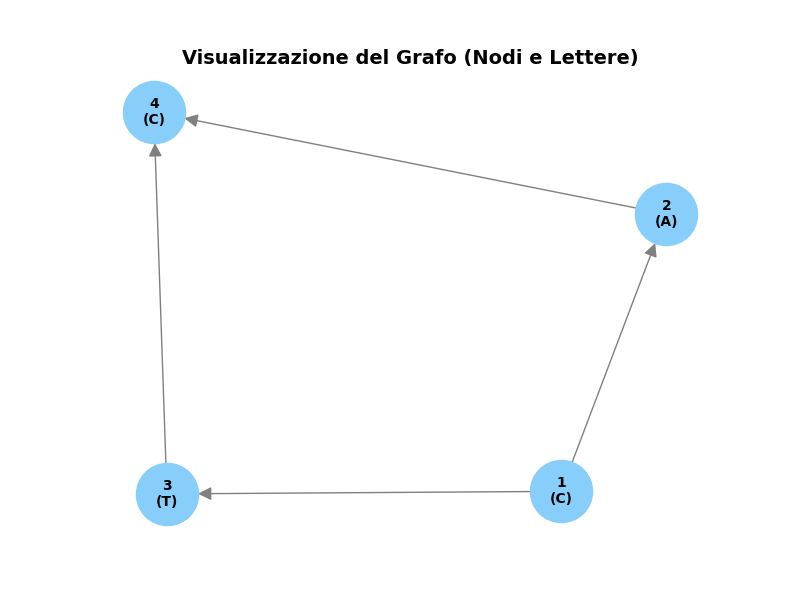
\includegraphics[width=0.7\textwidth]{IMG/GrafoOriginale.png}
    \caption{Grafo utilizzato per il Toy Example}
    \label{fig:Grafo originale}
\end{figure}


\begin{figure}[H]
    \centering
    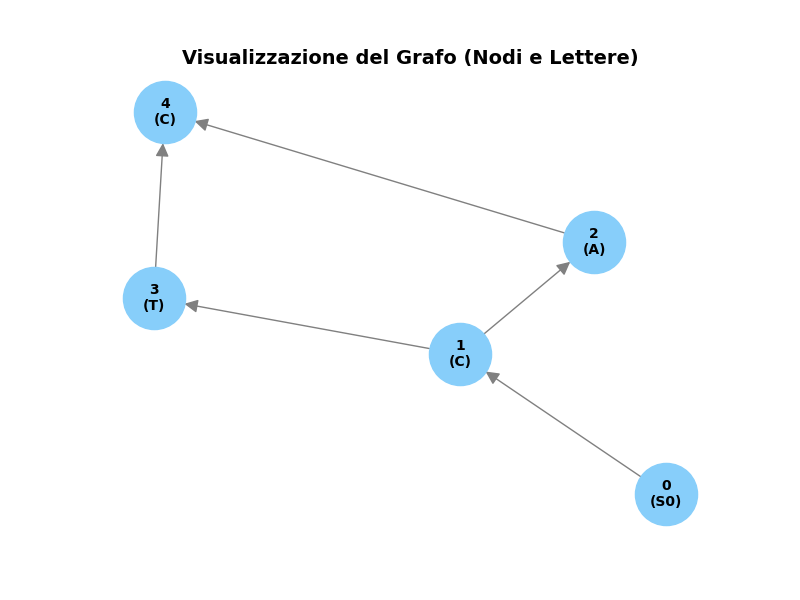
\includegraphics[width=0.7\textwidth]{IMG/Grafo.png}
    \caption{Grafo utilizzato per il Toy Example con nodo $S_0$ aggiunto}
    \label{fig:Grafo modificato}
\end{figure}




iniziamo a costruire la matrice ordinando i nodi topologicamente sulle colonne, il pattern andrà a occupare le righe, un carattere per riga.


\begin{table}[H]
    \centering
    \[
    \begin{array}{c|ccccc}
        & 0 & 1 & 3 & 2 & 4 \\
        & S0 & C & T & A & C \\
    \hline
    e &   &  &  &  &  \\
    C &   &  &  &  &   \\
    A &   &  &  &  &   \\
    C &  &  &  &  &   \\
    \end{array}
    \]
    \caption{Matrice delle distanze vuota}
    \label{tab:matrice-edit-toy-example-1}
\end{table}




Avviamo ora i primi passaggi andando a inserire i casi più semplici.
\\
\begin{itemize}
    \item $M[0,0] = 0$
    \item $M[i,0] = i \cdot 4, i < k+1$
    \item $M[0,v] = \min_{u \in Pred(v)} \{M[0,u] + g\}$
\end{itemize}



\begin{table}[H]
    \centering
    \[
    \begin{array}{c|ccccc}
        & 0 & 1 & 3 & 2 & 4 \\
        & S0 & C & T & A & C \\
    \hline
    e & 0  & 4 & 8 & 8 & 12 \\
    C & 4  &  &  &  &   \\
    A & 8  &  &  &  &   \\
    C & 12 &  &  &  &   \\
    \end{array}
    \]
    \caption{Matrice delle distanze con i primi casi eseguiti}
    \label{tab:matrice-edit-toy-example-2}
\end{table}




Eseguiamo ora i vari passaggi per riempire il resto delle celle
\begin{enumerate}
    \item Cella C-1(C): è un match di costo 1 (caratteri diversi da 'A'),
            la scelta di costo minimo è eseguire un match prelevando
            il valore della cella $M[0,0]$ che corrisponde al
            predecessore del nodo associato.
    \item Cella C-3(T): è un mismatch, costo 4, la scelta di costo
          minore è delezione, selezionamo il predecessore
          minore $M[C,3] = M[C,1] + g $
    \item Cella C-2(A): è un mismatch, costo 4, la scelta di costo
          minore è delezione, selezionamo il predecessore
          minore $M[C,2] = M[C,1] + g $
    \item Cella C-4(C): match (costo 1) e delezione pareggiano. Costo minimo: $\min(\{M[e,3], M[e,2]\}) + 1 = 8 + 1 = 9$.
    \item Cella A-1(C): mismatch (costo 4). Scelta minima, inserzione dall'alto: $M[C,1] + g = 1 + 4 = 5$.
    \item Cella A-3(T): mismatch (costo 4). Scelta minima, sostituzione dal predecessore 1: $M[C,1] + 4 = 1 + 4 = 5$.
    \item Cella A-2(A): match speciale (costo 0). Scelta minima, sostituzione dal predecessore 1: $M[C,1] + 0 = 1$.
    \item Cella A-4(C): mismatch (costo 4). Scelta minima, delezione dal predecessore 2: $M[A,2] + g = 1 + 4 = 5$.
    \item Cella C-1(C): match (costo 1). Scelta minima, sostituzione da $S0$ (o inserzione): $M[A,0] + 1 = 8 + 1 = 9$.
    \item Cella C-3(T): mismatch (costo 4). Scelta minima, sostituzione da nodo 1 o inserzione: $\min = 9$.
    \item Cella C-2(A): mismatch (costo 4). Scelta minima, inserzione dall'alto: $M[A,2] + g = 1 + 4 = 5$.
    \item Cella C-4(C): match (costo 1). Scelta minima, sostituzione dal predecessore 2: $M[A,2] + 1 = 1 + 1 = 2$.
\end{enumerate}


\begin{table}[H]
    \centering
    \[
    \begin{array}{c|ccccc}
        & 0 & 1 & 3 & 2 & 4 \\
        & S0 & C & T & A & C \\
    \hline
    e & 0  & 4 & 8 & 8 & 12 \\
    C & 4  & 1 & 5 & 5 & 9  \\
    A & 8  & 5 & 5 & 1 & 5  \\
    C & 12 & 9 & 9 & 5 & 2  \\
    \end{array}
    \]
    \caption{Matrice delle distanze di edit per il Toy Example}
    \label{tab:matrice-edit-toy-example}
\end{table}

La distanza di edit minima tra il pattern e il grafo è presente nella
cella $M[k+1,t+1]$.

/subsection{backtracking}
Per effettuare il backtraking viene usata una seconda matrice.
Tale matrice presenta in ogni cella [i,c] le cocordinate della cella da cui è stato 
prelevato il valore per calcolare il valore di tale cella.

La distanza di edit minima tra il pattern e il grafo è presente nell'ultima cella in basso a destra, ovvero $M[k, n]$.

\subsection{Backtracking}
Per effettuare il backtracking viene usata una seconda matrice.
Tale matrice presenta in ogni cella $M[i,c]$ le coordinate della cella da cui è stato prelevato il valore ottimale per calcolare il costo di tale mossa.

\begin{table}[H]
    \centering
    \[
    \begin{array}{cc|ccccc}
        &   & 0  & 1 & 3 & 2 & 4 \\
        &   & S0 & C & T & A & C \\
    \hline
    0 & e & (0,0) & (0,0) & (0,1) & (0,2) & (0,3) \\
    1 & C & (0,0) & (0,0) & (1,1) & (1,1) & (0,2) \\
    2 & A & (1,0) & (1,1) & (1,1) & (1,1) & (2,3) \\
    3 & C & (2,0) & (2,0) & (2,1) & (2,3) & (2,3) \\
    \end{array}
    \]
    \caption{Matrice di backtracking completa}
    \label{tab:matrice-backtracking-completa}
\end{table}
Una volta costruita la matrice dei puntatori, è sufficiente ripercorrere il cammino a ritroso a partire dalla cella finale. Ogni cella visitata contiene le coordinate della cella precedente a cui è necessario saltare; l'etichetta della colonna corrispondente indica il vertice del grafo da inserire nel cammino ottimo.

\end{document}